WWW:n, ja erityisesti WWW:n edeltäjän Gopherin, sivustot olivat alkujaan lähinnä staattisia dokumentteja, jotka oli linkitetty toisiinsa. Dokumentit muodostivat erillisia arkistoja esimerkiksi tutkijoiden käyttöön. Ajan kuluessa tuli tarpeelliseksi tehdä sivustoja, jotka reagoivat käyttäjän syötteeseen ja toimivat dynaamisesti käyttäjän syötteen mukaan.

Vuonna 1993 esitelty Common Gateway Interface (CGI) on standardi, jolla voidaan ajaa ohjelmia web-sivujen kautta UNIX-ympäristössä \cite{rfc3875}. Tyypillisesti CGI:llä ajettavat ohjelmat ovat itsenäisiä ja ne on kirjoitettu jollain skriptikielellä esimerkiksi Perlillä tai PHP:lla. Skripti saa parametrina käyttäjän lähettämät syötteet ja muodostaa sen perusteella käyttäjälle näkyvän HTML-sivun. Ajan kuluessa CGI-ohjelmat alkoivat kasvaa ja niiden arkkitehtuuri monimutkaistua, kun esimerkiksi niissä alettiin käyttää tietokantoja.

CGI-ohjelmien kasvun lisäksi myös niiden suoritukseen vaadittava ajoympäristö alkoi kasvaa ja muodostaa ongelmia CGI:n käytölle. CGI käynnistää suoritettavan prosessin jokaisen sivupyynnön yhteydessä, mikä voi olla hidasta, jos prosessi esimerkiksi lataa muistiin paljon dataa. Erityisesti 1990-luvulla Sunin kehittämä Java-kieli, joka saavutti suosiota web-kehittäjien keskuudessa, oli merkittävässä roolissa 1990-luvun lopun web-kehityksessä \cite{uml}.

Javan web-käyttöön suunniteltu Enterprise Edition (J2EE) käyttää Servlet-tekniikkaa, joka laajentaa perinteisen web-palvelimen toimintaa. Servlet-ohjelmia ei siis käynnistetä erillisestä web-palvelimesta, vaan se suoritetaan web-palvelimen sisällä. Käyttäjän pyynnön saatuaan web-palvelin (esimerkiksi Apache Tomcat) ohjaa pyynnön Java Servetille, joka käsiteltyään sen, palauttaa vastauksen web-palvelimelle, joka näyttää sivun käyttäjälle. Web-palvelin pitää siis Java-prosessia kokoajan käynnissä ja ympäristöä ei tarvitse käynnistää jokaisen käyttäjän pyynnön yhteydessä uudestaan. Servlet-tekniikan avulla voidaan tehostaa resurssien jakamista useamman pyynnön kesken, tehdä transaktioimalleja, muuttaa käyttäjäohjelman tilaa ja hallita web-sovelluksia etänä \cite{uml}. Eri kielille on toteutettu myös omia, Javan Servlettiä muistuttavia, web-palvelimia, esimerkiksi Ruby on Rails web-ohjelmointikehys tarjoaa oletuksena Rubyyn sisäänrakennetun WEBrick web-palvelimen, joka käynnistää ympäristön ja ohjaa pyynnöt oikeille Ruby on Rails -luokille \cite{ruby2011agile}. Kuvassa \ref{servlet} on kuvattu yksittäisen sivupyynnön kulkua Java Servlet-palvelimessa.

\begin{figure}[ht]
\centering
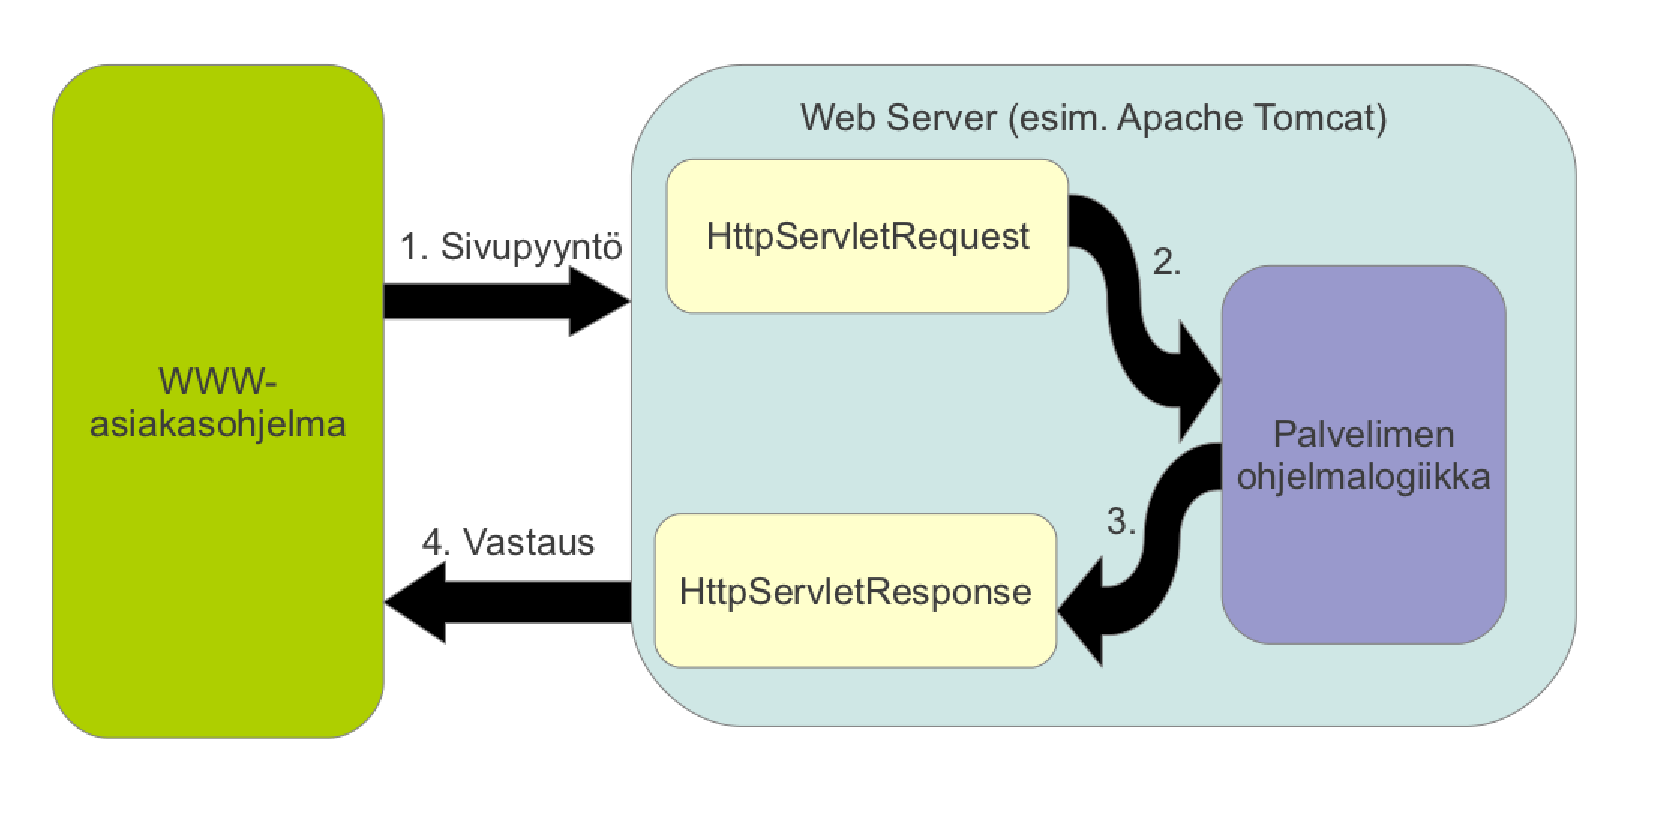
\includegraphics[width=\textwidth]{web/servlet.eps}
\caption{Kontrollin kulku Java Servlet-palvelimessa}%
\label{servlet}
\end{figure}

Servletien jälkeen paljon suosiota on saanut CGI:stä kehittynyt FastCGI-protokolla, joka korjaa CGI:ssä havaittuja puutteita \cite{fastcgi}. Web-palvelin ei käynnistä jokaista pyyntöä kohti uutta prosessia, vaan pyynnöt lähetetään ja vastaanotetaan pistokkeen (socket) avulla palvelimella suoritettavalle prosessille. FastCGI-ohjelmat voivat olla myös hajautettu eri palvelimille, jolloin pyyntöjen välitykseen käytetään TCP-yhteyttä. FastCGI:tä voidaan käyttää minkä tahansa kielen kanssa, joka tukee pistokkeiden käyttöä. Näin ollen se on varteenotettava tekniikka, koska ohjelmointikieli ei ole rajattu vain Javaan, vaan käytössä on Javan lisäksi koko kielien kirjo (esimerkiksi PHP, Python ja Ruby).

Tiivistetysti web-sovellusten historiasta voidaan sanoa, että niistä on tullut itsenäisiä ohjelmia, jotka pyörivät jatkuvasti palvelimella. Ohjelmat saavat kontrollin web-palvelimelta, joko laajentamalla web-palvelimen toimintaa (Servlet, WEBrick yms) tai pistokkeiden avulla (FastCGI). Web-sovellukset tuottavat käyttäjän syötteen ja web-sovelluksen sen hetkisen tilan mukaan käyttäjälle dynaamisen HTML tms muotoisen sivun. Seuraavissa kappaleissa pureudutaan web-sovellusten arkkitehtuuriin ja tutkitaan niiden kehitystä.